\section{Results}
\label{sec:results}

In this section we optimize a set of numerical programs using our tool in
a benchmark suite with six different examples.  We use the IEEE 754 32-bit
single precision format with rounding to nearest mode as the data types of the
floating-point values used in these examples.  The benchmark consists of two
introductory numerical programs, and four real applications that are frequently
encountered in numerical analyses, and round-off errors have big impacts on the
quality of their execution:
\begin{itemize}
    \item \texttt{simple}: for an input $x \in [0, 20]$, we repeatedly multiply
it with $0.9$, until the result is less than or equal to 1, the number of
iterations is dependent on $x$ and can only be determined by analyzing the
program.
    \item \texttt{basal}: the example in~\eqref{eq:syntax_example}.
    \item \texttt{taylor}: the Taylor expansion of $\cos(x + y)$, with single
precision inputs $x \in [-0.1, 0.1]$ and $y \in [0, 1]$, and an integer $n \in
[10, 20]$, which determines the bound on the iteration count.
    \item \texttt{filter}: computes the unit step response of a 3rd-order
infinite impulse response (IIR) filter, and all coefficients are bounded by
$[0.0, 0.2]$, and it has a fixed iteration count 20.
    \item \texttt{euler}, it uses Euler's method to solve the differential
equation of a harmonic oscillator $\ddot{x} + \omega^2 x = 0$, with both an
initial stationary position $x$ and $\omega^2$ bounded by $[0.0, 1.0]$, a step
size of $0.1$, and an iteration count $n \in [0, 20]$.  It returns the position
$x$ and velocity $\dot{x}$.
    \item \texttt{pid}, the example PID controller that was used as a case
study in~\cite{damouche14} as a motivation of automated accuracy optimization
of numerical programs, we make it more challenging by changing constant
coefficients to be bounds to model not only one, but a huge selection of PID
controllers, with $kp \in [9.0, 10.0]$, $ki \in [0.5, 0.7]$ and $kd \in [0,
3.0]$, and an iteration count $n \in [0, 20]$.
\end{itemize}

Our configuration for the efficient discovery of equivalent expressions
uses a depth limit $k = 2$, and a maximum 3 times of partial unrolling is
performed.  For each program we optimize it with our tool to discover a wide
range of implementations, and select the most accurate and least resource
demanding equivalent implementations for further analysis.  The selected
implementations are then simulated 1000 times, with a sample of 1000 unique
random inputs for each benchmark example, then we compare the maximum round-off
errors encountered.  Finally, our back-end transpiler produces C source codes
from MIRs, and they are synthesized with LegUp~\cite{legup}, an open source
HLS tool, with floating-point operator sharing turned off to achieve maximum
frequency, then compiled and verified with Quartus, targeting an Altera
Stratix IV device (EP4SGX530) for the actual resource usage statistics and the
frequency achieved.

Figure~\ref{fig:results} shows the results of optimizing the above benchmark
examples.  The rows labeled ``\texttt{FR}'' and ``\texttt{MA}'' respectively
show the statistics for the most resource efficient, and the most accurate
implementations.  ``Time (s)'' shows the time required for the optimization,
and ``PF'' shows the number of trade-off options in the Pareto frontier.  The
optimization runtime is longer than a typical compiler optimizer, because
during equivalent structure discovery, a significant amount of equivalent
structures are examined.  The values shown in the ``Error Bound'' column are
the maximum absolute errors found by our tool, while ``Simulation'' shows the
actual absolute value bound on round-off errors found during simulation, and
the percentage shows the actual accuracy improvement found in simulation of
``\texttt{MA}'' over ``\texttt{FR}''.  For each of these benchmark problems,
the optimization for accuracy of them translates well to the actual reduction
of simulated round-off errors in actual executions.  They all show improvements
in accuracy over the original by up to 65\% in actual execution.  The analyzed
round-off errors are larger than the simulated bounds, because our accuracy
analysis considers the worst case scenario, and the error bounds are computed
with the worst possible round-off error for each arithmetic computation,
whereas in actual computations worst case round-off errors are extremely rare.

\begin{figure}[ht]
    \centering
    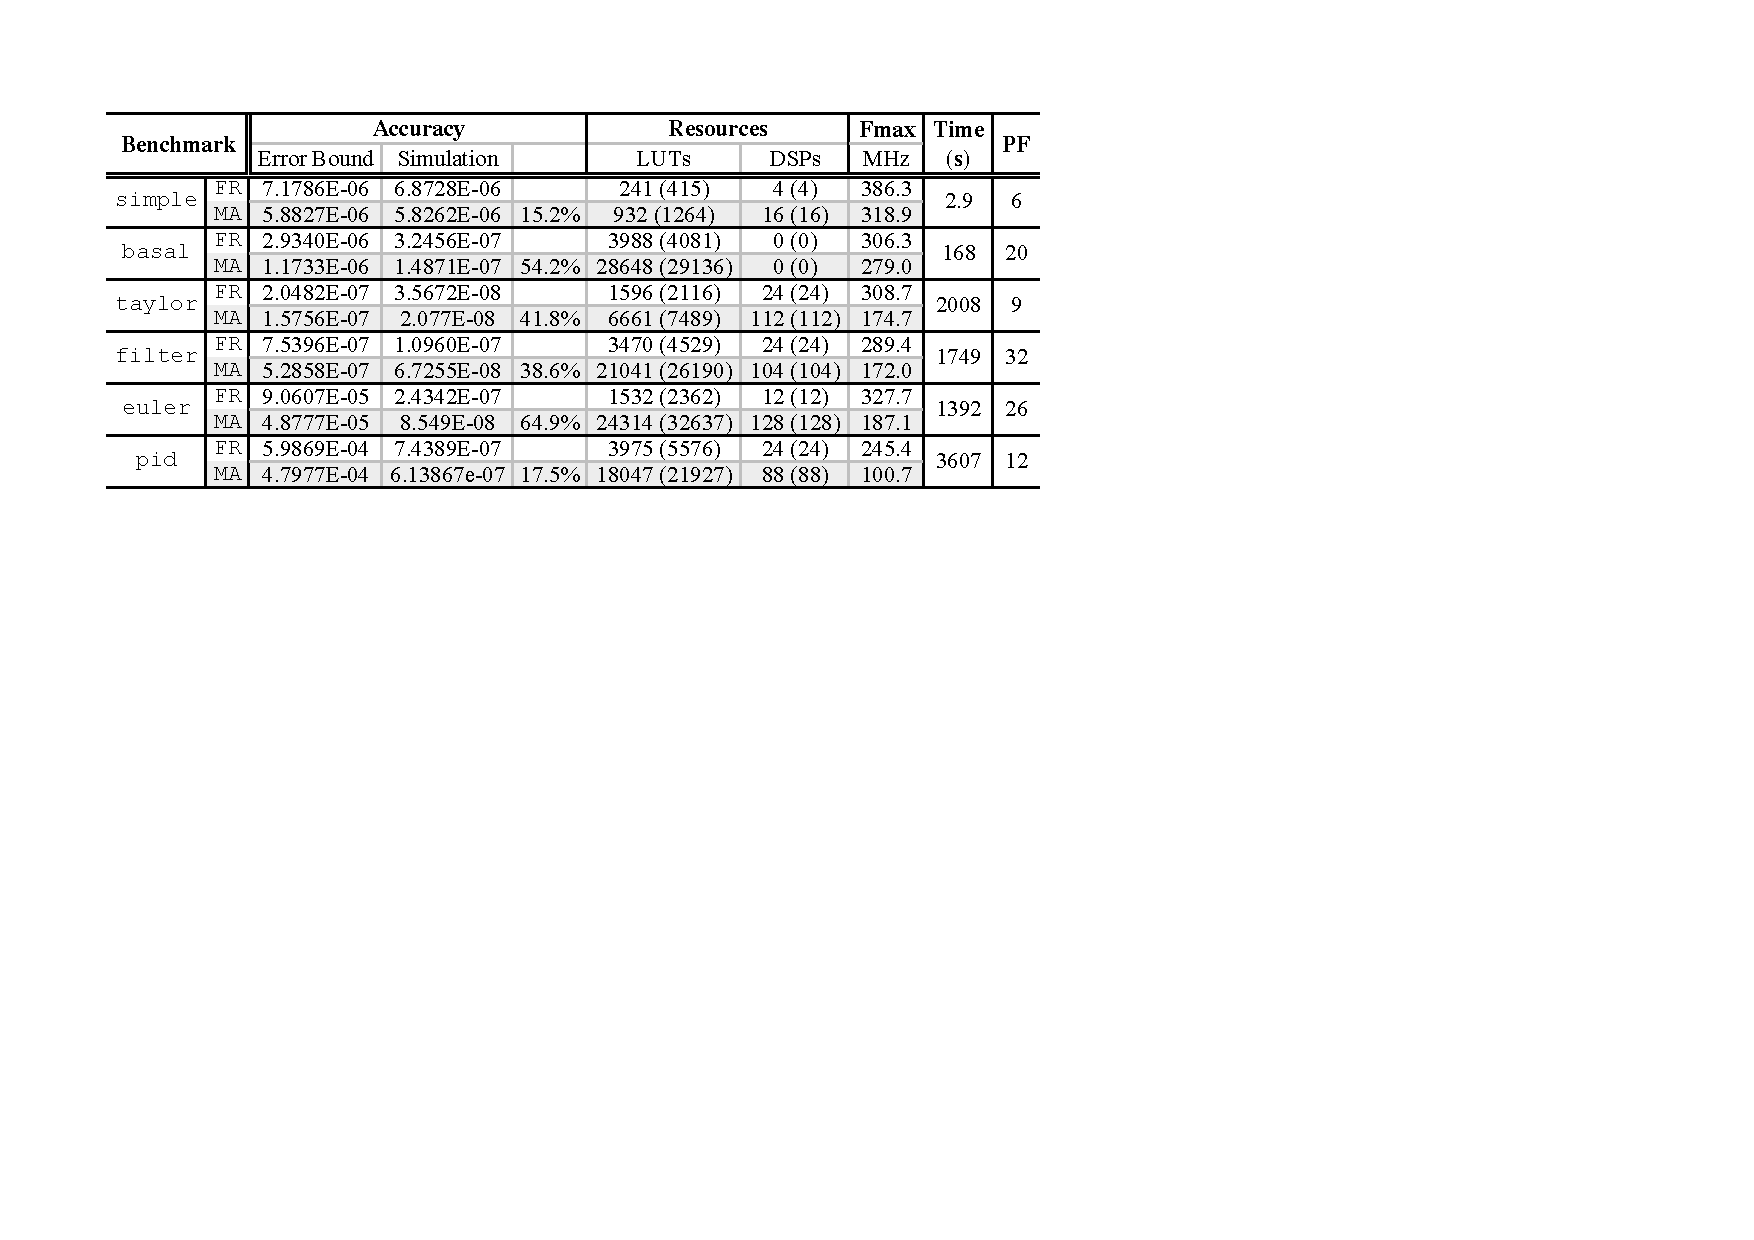
\includegraphics[width=\linewidth]{results}
    \captionof{figure}{%
    Table of optimization results.}\label{fig:results}
\end{figure}
\begin{figure}[ht]
    \centering
    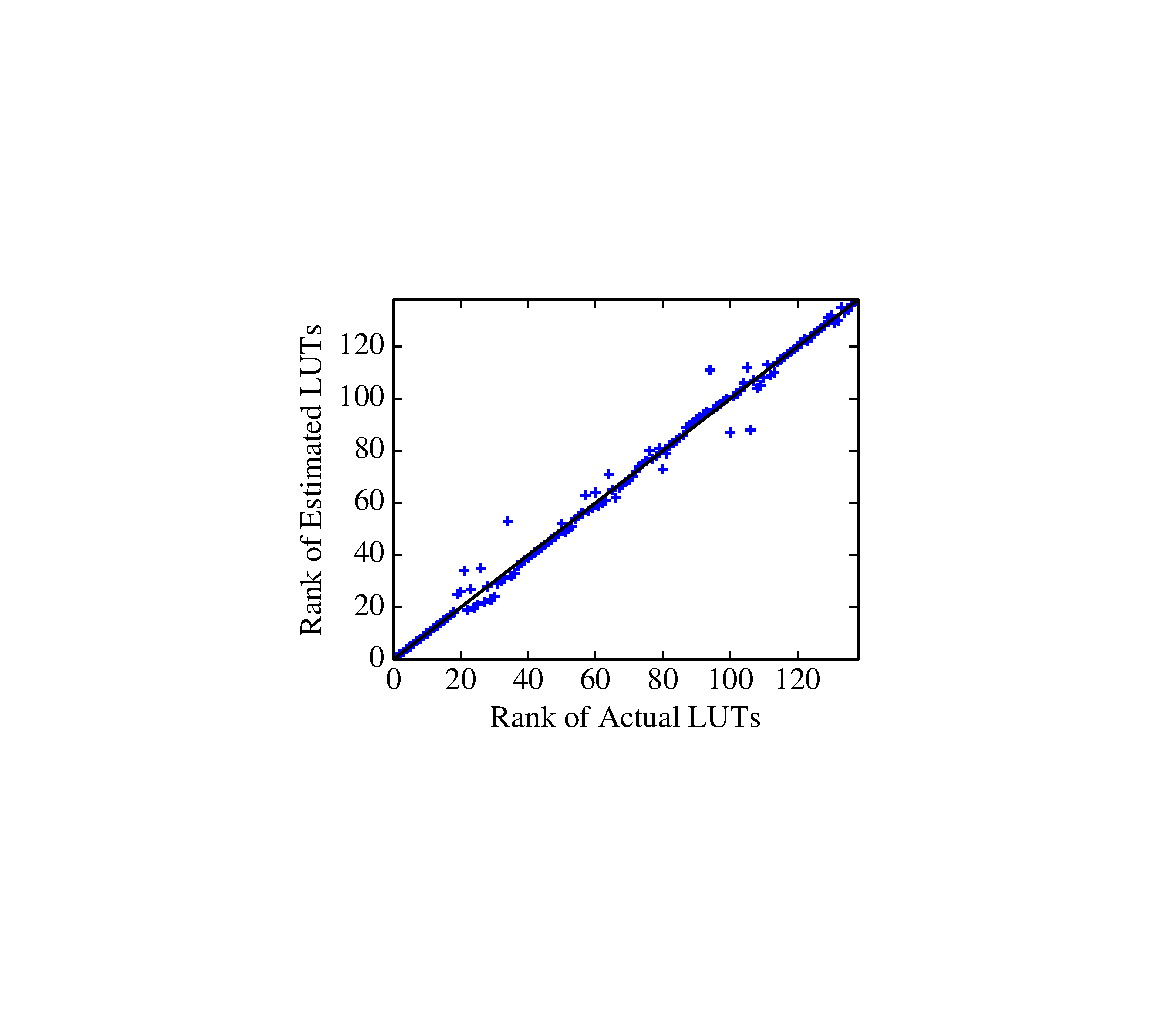
\includegraphics[scale=0.7]{rank}
    \captionof{figure}{%
    \mbox{The quality of resource estimation.}}\label{fig:rank}
\end{figure}

\begin{figure*}[ht]
    \centering
    \begin{minipage}{0.6\textwidth}
    \end{minipage}\quad\begin{minipage}{0.35\textwidth}
    \end{minipage}
\end{figure*}

The ``Resources'' columns show our estimation of the number of LUTs and
DSPs required for each of these programs, and the numbers in brackets are
the corresponding statistics obtained from Quartus synthesis.  Because
implementations on the Pareto frontier is only sensitive to how their LUTs
compare against each other, \ie~the rank, the Pareto frontier will not be
affected unless the rank is changed.  To ensure that the resource estimation
method used in our optimization can identify accurately whether an actual
implementations is on the Pareto frontier, we gathered 150 implementations
discovered across the benchmark examples, and for each one we rank its
number of estimated LUTs among them, and do the same for actual LUTs.
Figure~\ref{fig:rank} plots the rank of estimated LUTs against the rank of
actual LUTs, which shows the Pareto frontier we produced is very close to using
Quartus to count resources.

Because our benchmark examples are designed to be resource efficient, there
is no room for resource usage optimization of the original program.  However
we are able to consistently reduce the resource usage of a plain partial
loop unrolling by more than 25\%, because our optimization can discover
subexpression sharing opportunities, propagate constants values, and also
aggressively reduce the size of expressions by powerful reduction rules such as
$a - a = 0$ and $0 \times a = 0$.

Besides the choices of implementations that are either most accurate or most
resource efficient, each optimization also offers a wide selection of optimized
programs on the Pareto frontier.  For instance, Figure~\ref{fig:euler} shows
the Pareto frontier of \texttt{euler}, which has 26 different trade-off
options.  Furthermore, in the optimization of \texttt{euler}, our optimization
not only identifies that it is resource efficient when the two return variables
are computed by the same loop, but also by individually optimizing the
accuracy of the two variables, we produce a program with two loops, each with
a different goal, that is to compute their respective return variables as
accurately as possible, this generated a program that consists of two loops
that have completely different structures.  With this, we further widen the
trade-off curve with the most accurate option improving the accuracy by 65\%.
In Figure~\ref{fig:filter}, because the loop kernel of \texttt{filter} has the
expression $\sum_{i=0}^2{(a_i y_i + b_i x_i)}$, which has a large number of
equivalent expressions, without increasing the resource usage, our optimization
improves its accuracy by 14.5\%.  Because our Pareto frontier has three
dimensions, which are respectively accuracy, LUT utilization and the number of
DSPs, points within the shaded region optimize DSP count.

\begin{figure}[ht]
    \centering
    \subfloat[\texttt{euler}]{%
        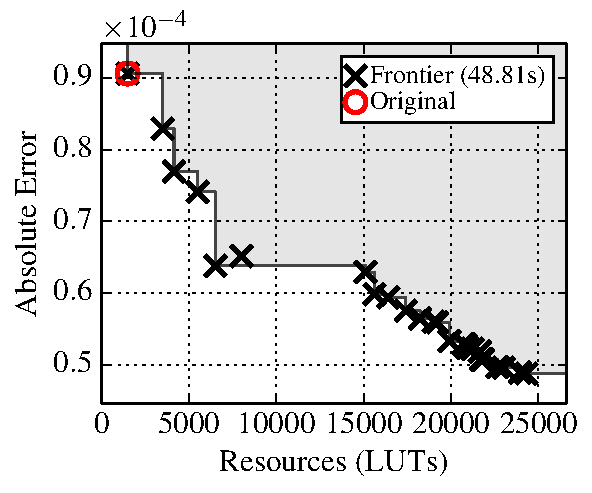
\includegraphics[width=0.6\linewidth]{euler}
        {}\label{fig:euler}
    } \\
    \subfloat[\texttt{filter}]{%
        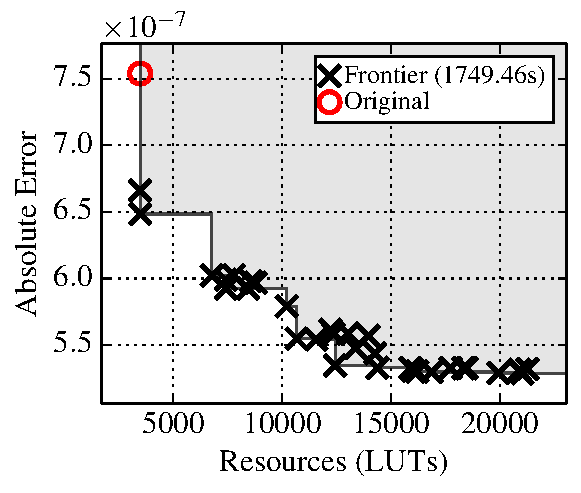
\includegraphics[width=0.6\linewidth]{filter}
        {}\label{fig:filter}
    }
    \caption{The Pareto frontier.}
\end{figure}
